\chapter{گزارش}
پروتکلی که طراحی و پیاده‌سازی شده به این صورت است که از طریق آن می‌خواهیم اطلاعات یک دانشجو که شامل شماره‌ی دانشجویی، نام دانشجو و رشته‌ی او است را منتقل کنیم.

ابتدا به کمک زبان 
\lr{ASN.1}
پروتکل مدنظر به شکل زیر پیاده شده‌است.

\begin{lstlisting}
	// main.asn1
	StudentModule DEFINITIONS ::=
	BEGIN
	
	Student ::= SEQUENCE {
		id INTEGER,
		name PrintableString,
		major PrintableString
	}
	
	END
\end{lstlisting}

به کمک کامپایلر 
\lr{asn1c}
کدهای مورد نیاز این پروتکل برای زبان‌های
\lr{C, CPP} 
تولید شده است که پوشه‌ی 
\lr{Sources} 
موجود اند.

سپس به کمک این موارد تولید شده یک کدگذار و یک کدگشا به کمک مدل
\lr{XER} 
پیاده‌سازی شده است.

\begin{lstlisting}
	// main.c
	#include <stdio.h>
	#include <sys/types.h>
	#include <Student.h>
	
	static int write_out(const void *buffer, size_t size, void *app_key) {
		FILE *out_fp = app_key;
		size_t wrote;
		wrote = fwrite(buffer, 1, size, out_fp);
		return (wrote == size) ? 0 : -1;
	}
	
	int encode(char *filename) {
		Student_t *student;
		student = calloc(1, sizeof(Student_t));
		
		student->id = 401725173;
		
		PrintableString_t name;
		OCTET_STRING_fromString(&name, "Ali Nazari");
		student->name = name;
		
		PrintableString_t major;
		OCTET_STRING_fromString(&major, "Computer Engineering");
		student->major = major;
		
		FILE *fp = fopen(filename, "wb");
		xer_encode(&asn_DEF_Student, student, XER_F_BASIC, write_out, fp);
		fclose(fp);
		
		fprintf(stderr, "Created %s with XER encoded Student\n", filename);
		xer_fprint(stdout, &asn_DEF_Student, student);
	}
	
	int decode(char *filename) {
		char buf[1024];     
		Student_t *student = 0;
		
		FILE *fp = fopen(filename, "rb");
		
		size_t size = fread(buf, 1, sizeof(buf), fp);
		fclose(fp);
		
		asn_dec_rval_t rval = xer_decode(0, &asn_DEF_Student, (void **)&student, buf, size);
		printf("Student ID: %d \t Name: %s \t Major: %s", 
		student->id, student->name.buf, student->major.buf);
	}
	
	int main(int ac, char **argv) {
		char *filename = "student.xml";
		
		char *command = argv[1];
		if (strcmp(command, "encode") == 0) {
			encode(filename);
		} else if (strcmp(command, "decode") == 0) {
			decode(filename);
		} else {
			printf("Please enter encode or decode");
		}
		
		return 0;
	}
\end{lstlisting}

با اجرای دستور 
\lr{./run.sh encode}
قطعه کد مربوط به کدگذار اجرا می‌شود و پس از کدگذاری، خروجی را در فایل 
\lr{student.xml} 
ذخیره می‌کند.

\begin{figure}[H]
	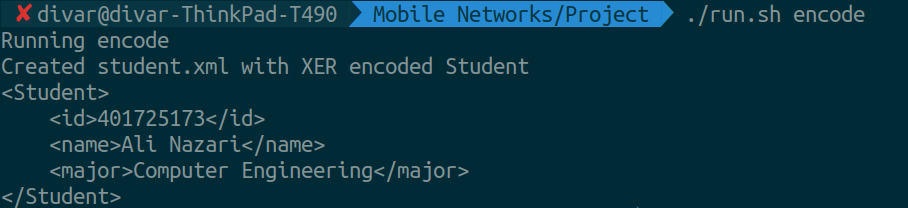
\includegraphics[width=0.85\columnwidth]{Picture/encode.png}
	\centering
	\caption{اجرای کدگذار}
\end{figure}

هم‌چنین با اجرای دستور 
\lr{./run.sh decode}
قطعه کد مربوط به کدگشا اجرا می‌شود و فایل ذخیره شده را خوانده و عملیات کدگشایی را انجام می‌دهد.

\begin{figure}[H]
	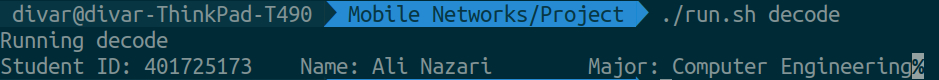
\includegraphics[width=0.85\columnwidth]{Picture/decode.png}
	\centering
	\caption{اجرای کدگشا}
\end{figure}
